\documentclass[letterpaper, 12pt]{math}

\usepackage{forest}
\usepackage{pgfplots}

\title{CSCI 251: Concepts of Parallel and Distributed Systems}
\author{Alvin Lin}
\date{August 30th, 2017}

\begin{document}

\maketitle

\section*{Topics}
\begin{itemize}
  \item Parallel Addition
  \item Speed up
  \item Amdahl's Law
  \item Efficiency
  \item Scalability
  \item Superlinear speedup
  \item Merge Sort
\end{itemize}

\subsection*{Parallel Addition}
Suppose we have N numbers to add. A serial computation would require (N-1)
additions, making it an \( O(N) \) operation. If we were to add N numbers
2 at a time in a tree structure like manner, then it would only take
\( \log_{2}N \) steps.
\begin{center}
  \begin{forest}
    [\( \sum_{1}^{8}d_{i} \)
      [\( \sum_{1}^{4}d_{i} \)
        [\( d_{1}+d_{2} \)
          [\( d_{1} \)]
          [\( d_{2} \)]
        ]
        [\( d_{3}+d_{4} \)
          [\( d_{3} \)]
          [\( d_{4} \)]
        ]
      ]
      [\( \sum_{5}^{8}d_{i} \)
        [\( d_{5}+d_{6} \)
          [\( d_{5} \)]
          [\( d_{6} \)]
        ]
        [\( d_{7}+d_{8}\)
          [\( d_{7} \)]
          [\( d_{8} \)]
        ]
      ]
    ]
  \end{forest}
\end{center}

\subsection*{Speed Up}
The speed up is the time taken to execute a given problem on a single computer
over the time take to execute the given problem on a parallel computer. We
make several assumptions about the parallel computer:
\begin{itemize}
  \item each processor runs on the same clock speed
  \item the bandwidth is the same for all communications
  \item the memory access times are the same
\end{itemize}

\subsubsection*{Message Passing Model}
Each of the steps in the tree above requires a communication step as well as
the addition operation.
\begin{align*}
  d_{1} & \leftarrow & d_{2} && d_{3} & \leftarrow & d_{4} && d_{5}
    & \leftarrow & d_{6} && d_{7} & \leftarrow & d_{8} \\
  P_{1} && P_{2} && P_{3} && P_{4} && P_{5} && P_{6} && P_{7} && P_{8} \\ \\
  d_{1}+d_{2} & \leftarrow & d_{3}+d_{4} && d_{5}+d_{6} & \leftarrow &
    d_{7}+d_{8} \\
  \dots
\end{align*}
Even numbered processors will pass a message to \( P_{i-1} \).

\subsubsection*{Shared Memory Model}
Alternatively, there can exist a region of shared memory which all processors
\( P_{i} \) can access. During the communication step, each processor
\( P_{i} \) writes \( d_{i} \) into shared memory. The flow will be as follows:
\begin{itemize}
  \item memory write
  \item memory read
  \item add
  \item memory write
\end{itemize}
There needs to be a mechanism (mutex lock/semaphore) to make the shared memory
operations atomic.

\subsection*{Modeling the speed up}
The speed up is limited by the portion of the program that can be parallelized.
Suppose in a given problem, \( \alpha \) is the portion that cannot be
parallelized. \( (1-\alpha) \) is the portion that can be parallelized.
Given that the time taken to execute the algorithm on a single computer is
\( T_{s} = 1 \), the time taken to execute the same algorithm on a parallel
computer with \( P \) processors is given by:
\[ T_{p} = \frac{1-\alpha}{P}+\alpha \]
The speed up \( S \) is given by:
\begin{align*}
  S &= \frac{T_{s}}{T_{p}} \\
  &= \frac{1}{\frac{1-\alpha}{P}+\alpha}
\end{align*}

\subsection*{Amdahl's Law}
This speed is bounded by \( \frac{1}{\alpha} \), thus you cannot get a speed up
greater than \( \frac{1}{\alpha} \). Suppose \( \alpha = 0.2 \), meaning 20\%
of the program cannot be parallelized. With 2 processors:
\[ S = \frac{1}{\frac{0.8}{2}+0.2} = \frac{1}{0.6} = \frac{5}{3} \]
With \( P = 4 \):
\[ S = \frac{1}{\frac{0.8}{4}+0.2} = \frac{1}{0.4} = 2.5 \]
With \( P = 8 \):
\[ S = \frac{1}{0.3} = 3.33 \]
Graphing this, we can see the limitations of the speed up in that it is
upper bounded by \( \frac{1}{\alpha} \):
\begin{center}
  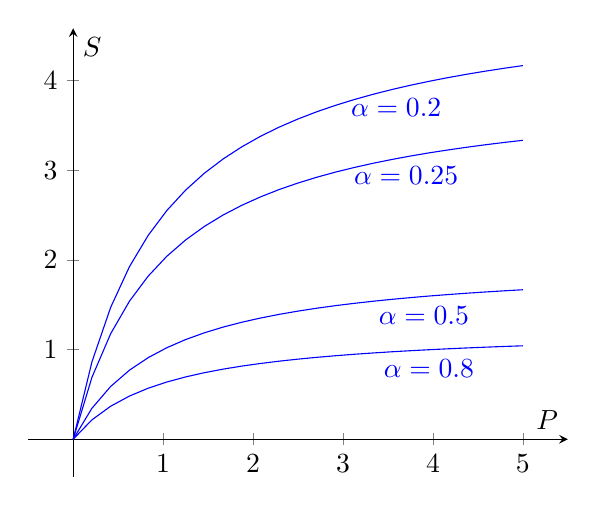
\begin{tikzpicture}
    \begin{axis}[axis lines=middle,
                 xlabel=\( P \), ylabel=\( S \),
                 enlargelimits]
      \addplot[blue,
               domain={0:5}]{1/((0.2/x)+0.2)} node[pos=0.8, below]
               {\( \alpha = 0.2 \)};
      \addplot[blue,
               domain={0:5}]{1/((0.25/x)+0.25)} node[pos=0.8, below]
               {\( \alpha = 0.25 \)};
      \addplot[blue,
               domain={0:5}]{1/((0.5/x)+0.5)} node[pos=0.8, below]
               {\( \alpha = 0.5 \)};
      \addplot[blue,
               domain={0:5}]{1/((0.8/x)+0.8)} node[pos=0.8, below]
               {\( \alpha = 0.8 \)};
   \end{axis}
 \end{tikzpicture}
\end{center}

\subsection*{Efficiency}
The efficiency \( E \) is equal to the speed up \( S \) over the number of
processors \( P \):
\begin{align*}
  E &= \frac{S}{P} \\
  &= \bigg[\frac{1}{\frac{1-\alpha}{P}+\alpha}\bigg]\frac{1}{P}
\end{align*}

\subsection*{Scalability}
In the initial addition problem, \( N \) was equal to \( P \). In real world
situations, \( N \) is often far greater than \( P \). For \( N = 64 \) and
\( P = 4 \), each processor should get \( \frac{N}{P} \) data elements.
\begin{align*}
  P_{1} &\rightarrow \sum_{1}^{16}d_{i} \\
  P_{2} &\rightarrow \sum_{17}^{32}d_{i} \\
  P_{3} &\rightarrow \sum_{33}^{48}d_{i} \\
  P_{4} &\rightarrow \sum_{49}^{64}d_{i}
\end{align*}
\( \frac{N}{P}-1 \) additions on each processor is \( O(\frac{N}{P}) \)
with \( \log_{2}P \) steps, or \( O(\frac{N}{P}+\log(P)) \).

\subsection*{Superlinear speedup}
Depth-First Search Trees, search time can be halved by dividing the task
between two computers.

\subsection*{Reminders}
Professor Mohan Kumar: \\
\url{mjkvcs@rit.edu} \\
\url{https://cs.rit.edu/~mjk} \\

\noindent Jennifer Burt (Additional Contact): \\
\url{jennifer@cs.rit.edu}

\subsection*{Homework}
Check MyCourses for sample questions. There will be a small quiz in class
next Wednesday.

\begin{center}
  You can find all my notes at \url{http://omgimanerd.tech/notes}. If you have
  any questions, comments, or concerns, please contact me at
  alvin@omgimanerd.tech
\end{center}

\end{document}
